\documentclass[a4paper,12pt]{article}
\usepackage[utf8]{inputenc}
\usepackage[T2A]{fontenc}
\usepackage[russian]{babel}
\usepackage{graphicx}
\usepackage{amsmath,amsfonts,amssymb}
\usepackage{geometry}
\geometry{top=2cm, bottom=2cm, left=2.5cm, right=1.5cm}
\usepackage{indentfirst}
\usepackage{multirow}
\usepackage{booktabs}
\usepackage{caption}
\usepackage{pgfplots}
\pgfplotsset{compat=1.18}
\usepackage{tikz}
\usetikzlibrary{patterns}
\usepackage{setspace}
\onehalfspacing
\usepackage{siunitx} % Для красивых единиц измерения

% Красивые заголовки
\usepackage{titlesec}
\titleformat{\section}{\Large\bfseries\sffamily}{\thesection}{1em}{}
\titleformat{\subsection}{\bfseries\sffamily}{\thesubsection}{1em}{}
\titleformat{\subsubsection}{\bfseries\sffamily}{\thesubsubsection}{1em}{}

% Для имитации рукописного шрифта в титуле (опционально)
\usepackage{aurical}
\usepackage{color}

\begin{document}

% Титульный лист
\begin{titlepage}
    \begin{center}
        % Верхняя часть с названием вуза
        \textbf{МОСКОВСКИЙ ФИЗИКО-ТЕХНИЧЕСКИЙ ИНСТИТУТ} \\
        \textbf{(НАЦИОНАЛЬНЫЙ ИССЛЕДОВАТЕЛЬСКИЙ УНИВЕРСИТЕТ)}
        \\[1cm]

        
        % Название факультета (чуть меньше)
        {\large Физтех-школа аэрокосмических технологий}
        \\[3.5cm]

        % Самое большое — полное название работы
        {\Huge \textbf{Гидродинамическая устойчивость}}
        \\[0.5cm]
        {\Huge \textbf{вращательного течения Куэтта}}
        \\[10cm]

        % Блок с именами и группами (выравнивание по правому краю)
        \begin{flushright}
            \begin{tabular}{l l}
                Копышова Валентина Олеговна & Б03-3046 \\
                Ларькин Глеб Сергеевич & Б03-301а \\
                Дай Сюй                  & Б03-3046 \\
                Ордоньес Эррера Хулио Себастьян & Б03-3046 \\
            \end{tabular}
        \end{flushright}

        \vfill

        % Нижняя часть
        {\large Долгопрудный, 2026 г.}
    \end{center}
\end{titlepage}

\tableofcontents
\newpage

\section{Введение}
Течение Куэтта представляет собой движение вязкой жидкости в зазоре между двумя коаксиальными цилиндрами. В зависимости от направлений и величин угловых скоростей вращения цилиндров, течение может быть устойчивым или неустойчивым - переходить в режим с ярко выраженными структурами (вихрями Тейлора), а затем в турбулентный.



Переход от одного режима к другому определяется безразмерными параметрами — числами Рейнольдса для каждого цилиндра:
\[
Re_i = \frac{\Omega_i R_i^2}{\nu},
\]
где \(\Omega_i\) — угловая скорость, \(R_i\) — радиус цилиндра (\(i=1\) для внутреннего, \(i=2\) для внешнего), \(\nu\) — коэффициент кинематической вязкости жидкости.

\section{Теоретическая часть}

\subsection{Стационарное распределение скоростей}
Рассмотрим вязкую жидкость, заполняющую пространство между двумя цилиндрами с радиусами \(R_1\) и \(R_2\) (\(R_1 < R_2\)), вращающимися с угловыми скоростями \(\Omega_1\) и \(\Omega_2\). В стационарном состоянии, когда течение ламинарно и осесимметрично (\(u_r = 0, u_z = 0, u_\theta = V(r)\)), уравнения Навье-Стокса в цилиндрических координатах сводятся к уравнению :
\begin{equation}
\frac{1}{r} \frac{d}{dr}\left(r \frac{dV}{dr}\right) - \frac{V}{r^2} = 0.
\label{eq:stationary}
\end{equation}
Решение этого уравнения ищется в виде \(V(r) = Ar + B/r\). Угловая скорость жидкости \(\Omega(r) = V(r)/r\) тогда равна:
\begin{equation}
\Omega(r) = A + \frac{B}{r^2}.
\label{eq:omega}
\end{equation}
Константы \(A\) и \(B\) находятся из граничных условий прилипания на стенках цилиндров (\(\Omega(R_1) = \Omega_1\), \(\Omega(R_2) = \Omega_2\)):
\begin{equation}
A = \frac{\Omega_2 R_2^2 - \Omega_1 R_1^2}{R_2^2 - R_1^2}, \quad B = \frac{(\Omega_1 - \Omega_2) R_1^2 R_2^2}{R_2^2 - R_1^2}.
\label{eq:AB}
\end{equation}

\subsection{Устойчивость движения невязкой жидкости, критерий Релея}
Для идеальной (невязкой) жидкости условие устойчивости было получено Релеем на основе анализа сохранения момента импульса. При малом радиальном смещении элемента жидкости из положения равновесия возвращающая сила возникает, если квадрат циркуляции скорости \(\mu = r^2\Omega(r)\) возрастает с радиусом. Критерий Релея для устойчивости течения Куэтта в невязкой жидкости имеет вид:
\begin{equation}
\frac{d}{dr}\mu^2 = \frac{d}{dr}(r^2\Omega(r))^2 > 0.
\label{eq:rayleigh}
\end{equation}
Подставляя решение (\ref{eq:omega}), получаем условие:
\begin{equation}
\Omega(r)(\Omega_2 R_2^2 - \Omega_1 R_1^2) > 0.
\label{eq:rayleigh_cond}
\end{equation}
Из этого условия следует, что:
\begin{itemize}
    \item Если цилиндры вращаются в противоположные стороны, \(\Omega(r)\) меняет знак внутри зазора, и условие (\ref{eq:rayleigh_cond}) не выполняется. Такое течение всегда неустойчиво по отношению к малым возмущениям в рамках невязкой модели.
    \item Если цилиндры вращаются в одну сторону, то условие устойчивости эквивалентно \(\Omega_2 R_2^2 > \Omega_1 R_1^2\).
\end{itemize}
Граница устойчивости для невязкой жидкости в плоскости параметров (\(\Omega_1, \Omega_2\)) представляет собой прямую \(\Omega_2 R_2^2 = \Omega_1 R_1^2\) (см. Рис. 20.5 в лабораторном практикуме).

\subsection{Устойчивость движения вязкой жидкости: число Тейлора}
Вязкость оказывает стабилизирующее влияние, сдвигая границу устойчивости по сравнению с предсказаниями теории невязкой жидкости. Для теоретического исследования устойчивости вязкого течения Куэтта используется метод малых возмущений. На стационарное решение накладываются малые осесимметричные возмущения вида \(e^{\gamma t + ikz}\). В результате линеаризации уравнений Навье-Стокса получается система уравнений для амплитуд возмущений. Анализ показывает, что ключевым безразмерным параметром, определяющим устойчивость, является число Тейлора (\(Ta\)):
\begin{equation}
Ta = -\frac{4AB}{\nu^2} R_2^4 = \frac{4\Omega_1^2 R_1^4}{\nu^2} \cdot \frac{(1 - \mu)(1 - \mu/\eta^2)}{(1 - \eta^2)^2}.
\label{eq:Taylor}
\end{equation}
Здесь \(\mu = \Omega_2/\Omega_1\) — отношение угловых скоростей, а \(\eta = R_1/R_2\) — отношение радиусов. Нейтральная кривая \(\gamma(k) = 0\) в пространстве параметров (\(Ta, k\)) определяет границу устойчивости. Минимальное значение \(Ta\), при котором появляются нарастающие возмущения, называется критическим числом Тейлора \(Ta_{cr}\).

Для случая узкого зазора (\(d = R_2-R_1 \ll R_1\)) Тейлор получил аналитическое выражение для нейтральной кривой:
\begin{equation}
Ta = \frac{2(\pi^2 + a^2)^3}{a^2(2 + \alpha)} \left[ 1 - \frac{16a\pi^2 \cosh^2(a/2)}{(\pi^2 + a^2)^2(a + \sinh a)} \right]^{-1},
\label{eq:taylor_narrow}
\end{equation}
где \(a = kd\) — безразмерное волновое число, \(\alpha = -(1-\mu)\). Минимум этого выражения дает критическое число Тейлора:
\begin{equation}
Ta_{cr} = \frac{3430}{2 + \alpha}, \quad a_{cr} \approx 3.12.
\label{eq:taylor_crit}
\end{equation}
Зная \(Ta_{cr}\) для заданного \(\mu\), можно вычислить критические числа Рейнольдса для внутреннего и внешнего цилиндров:
\begin{equation}
Re_{1,cr} = \frac{\Omega_{1,cr} R_1^2}{\nu}, \quad Re_{2,cr} = \frac{\Omega_{2,cr} R_2^2}{\nu}.
\label{eq:Re_crit}
\end{equation}
Подставляя \(\Omega_{1,cr}\) из определения \(Ta\), можно построить теоретическую границу устойчивости в плоскости (\(Re_1, Re_2\)), как показано на графике ниже.

\newpage
\section{Экспериментальная установка и методика}
Установка состоит из двух коаксиально расположенных цилиндров: внутреннего (из непрозрачного дюраминилия) и внешнего (из прозрачного оргстекла), - радиусов  \(R_1 = 3.0 \text{см}\) и \(R_2 = 3.5 \text{см}\) соответсвтенно. Пространство между ними заполнено конденсаторным маслом с добавлением алюминиевой пудры. Частицы пудры, имеющие продолговатую форму, ориентируются вдоль линий тока, что позволяет визуализировать структуру течения.

Каждый цилиндр приводится во вращение отдельным электродвигателем с независимой регулировкой частоты вращения. Частота вращения задается звуковыми генераторами и измеряется с помощью оптических датчиков и частотомеров. На роторе каждого двигателя установлен диск со 100 отверстиями, что позволяет измерять частоту вращения \(f\) в об/с. Кинематическая вязкость масла известна из справочных данных и считается постоянной: \(\nu = \SI{2e-5}{\square\meter\per\second}\) (с погрешностью до 5\%).

Методика эксперимента заключается в плавном увеличении частоты вращения одного (или обоих) цилиндров до момента появления устойчивых тороидальных вихрей, видимых невооруженным глазом. Фиксируются частоты \(f_1\) и \(f_2\), соответствующие разному количеству вихрей.

\textbf{Стоит отметить, что в нашем случае частотомер, связанный с внешним цилиндром, вел себя некорретно, из-за чего оценка частоты его вращения происходила иными, менее точными, методами.}

\newpage
\section{Ход работы}
Эксперимент проводился в трёх режимах:
\begin{enumerate}
    \item Внешний цилиндр неподвижен (\(f_2 = 0\)).
    \item Внешний цилиндр вращается с малой постоянной скоростью (\(\sim 1 \text{Гц}\)).
    \item Цилиндры вращаются в противоположные стороны (данные для одного режима).
\end{enumerate}
В каждом режиме определялись частоты вращения внутреннего цилиндра, при которых появлялись устойчивые вихри. В режиме 2 также измерялась частота вращения внешнего цилиндра, вращение которого с постоянной скоростью обеспечить не удалось.

Ниже представлены фотографии получившихся вихрей Тейлора - слева случай параллельного вращения цилиндров (один набор вихрей), справа случай вращения цилиндров в противоположные стороны.

\textsl{В режиме 3 (вращение в противоположные стороны) скорость течения в какой-то момент меняет знак => существует поверхность нулевой скорости. Тогда можно заменить исходную задачу на две независимые, где одна стенка цилиндра вращается, а вторая покоится => будет два набора вихрей.}

\textsl{Для образования двух наборов вихрей важно, чтобы расстояния между поверхностью нулевой скорости и поверхностями цилиндров (внутренним и внешним) соотносились как 1:1.}

\begin{figure}[h]
\begin{tabular}{ll}
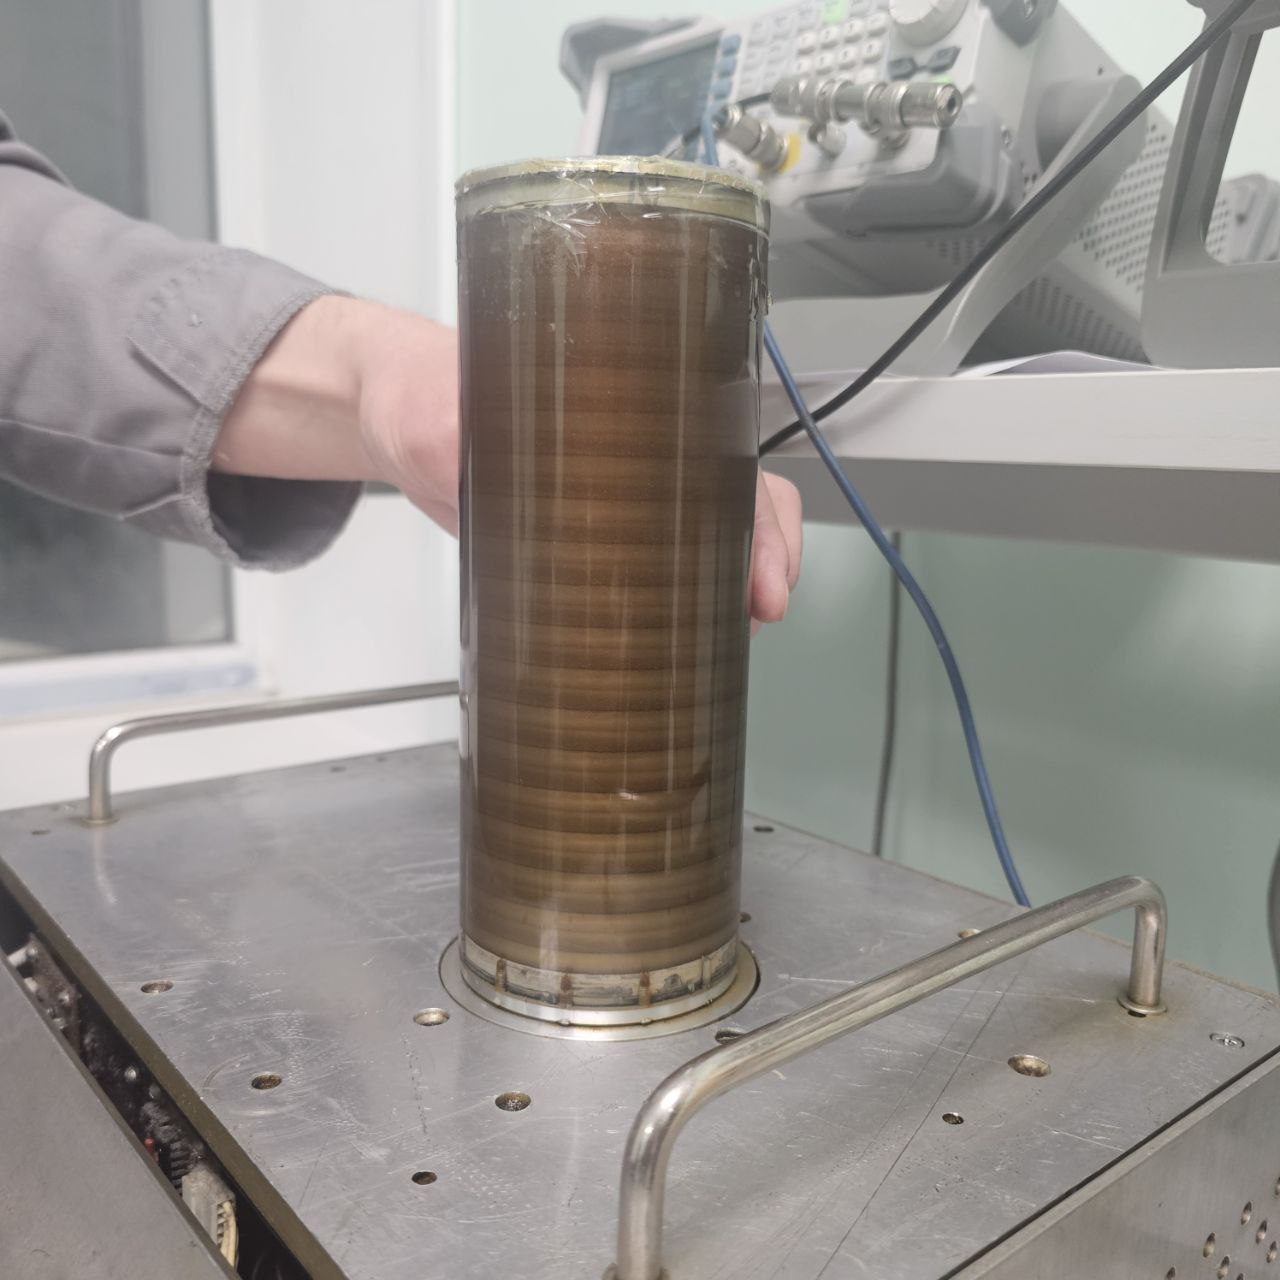
\includegraphics[scale=0.2]{photoes/one_Taylor_vortex.jpg}
&
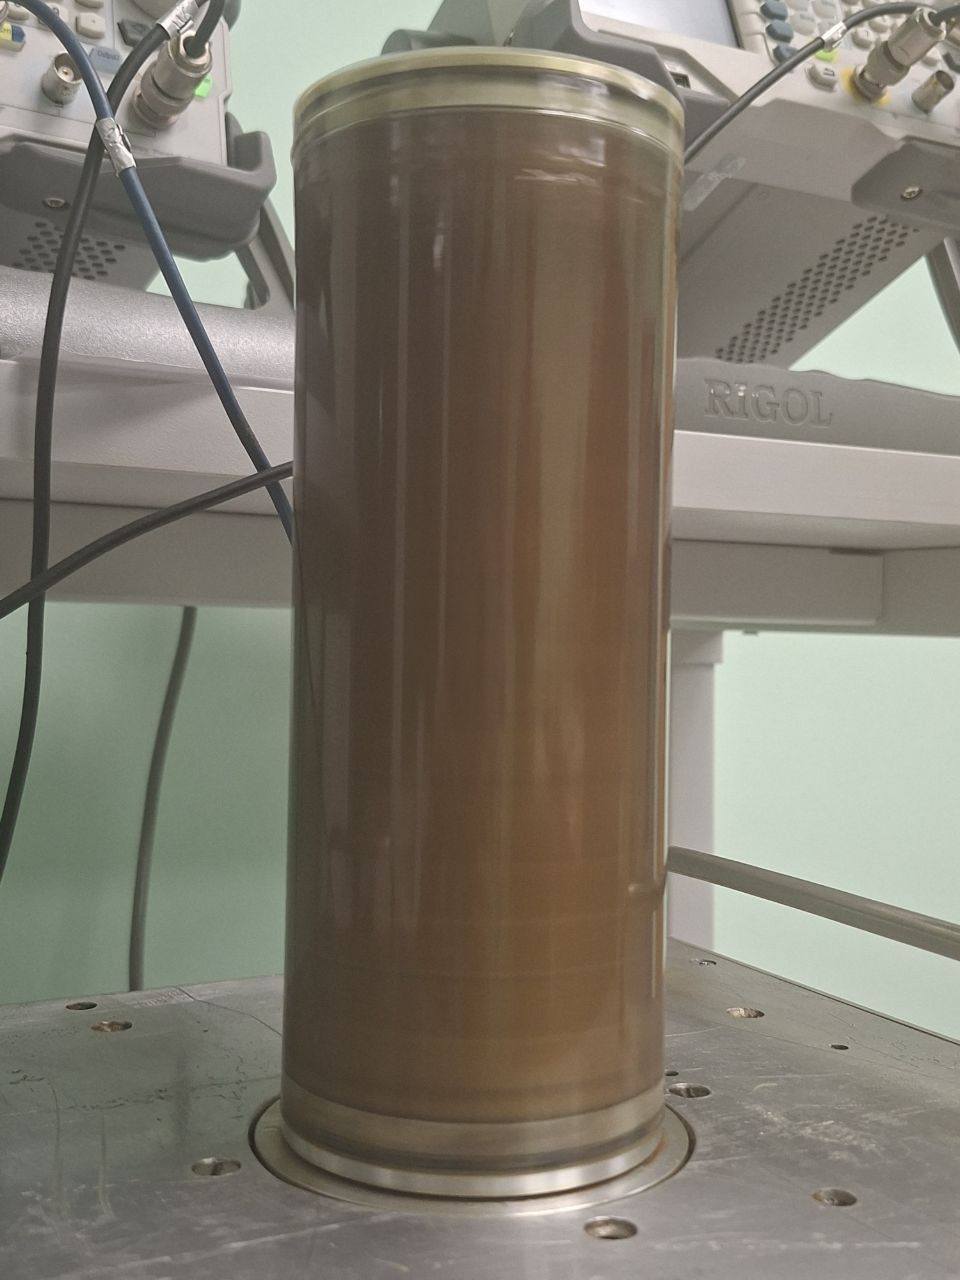
\includegraphics[scale=0.2]{photoes/two_Taylor_vortex.jpg}
\end{tabular}
\caption{Фотографией вихрей Тейлора}
\label{Fig:Race}
\end{figure}

% \subsection{Измеренные частоты и количество вихрей}

% \begin{table}[h!]
%     \centering
%     \caption{Режим 1: Внешний цилиндр неподвижен.}
%     \begin{tabular}{|c|c|}
%         \hline
%         Число вихрей & Частота внутреннего цилиндра \(f_1\), Гц \\
%         \hline
%         3 & 5.7 \\
%         10 & 8.0 \\
%         14 & 8.1 \\
%         20 & 8.3 \\
%         24 & 8.6 \\
%         34 & 8.8 \\
%         \hline
%     \end{tabular}
%     \label{tab:mode1}
% \end{table}

% \begin{table}[h!]
%     \centering
%     \caption{Режим 2: Внешний цилиндр вращается с частотой \(\approx \SI{1}{Гц}\). Измеренные частоты вращения внутреннего цилиндра.}
%     \begin{tabular}{|c|c|}
%         \hline
%         Число вихрей & Частота внутреннего цилиндра \(f_1\), Гц \\
%         \hline
%         3 & 8.8 \\
%         12 & 9.5 \\
%         18 & 9.9 \\
%         2 & 9.9 \\
%         36 & 10.0 \\
%         \hline
%     \end{tabular}
%     \label{tab:mode2}
% \end{table}

% \begin{table}[h!]
%     \centering
%     \caption{Режим 3: Внешний цилиндр не зафиксирован, вращается под действием потока.}
%     \begin{tabular}{|c|c|}
%         \hline
%         Частота внутреннего \(f_1\), имп/с & Частота внешнего \(f_2\), имп/с \\
%         \hline
%         1070 & 585 \\
%         1135 & 616 \\
%         1151 & 631 \\
%         1183 & 645 \\
%         1230 & 673 \\
%         1276 & 700 \\
%         1292 & 710 \\
%         \hline
%     \end{tabular}
%     \label{tab:mode3}
% \end{table}

% \begin{table}[h!]
%     \centering
%     \caption{Режим 4: Противонаправленное вращение.}
%     \begin{tabular}{|c|c|}
%         \hline
%         Частота внутреннего \(f_1\), имп/с & Частота внешнего \(f_2\), имп/с \\
%         \hline
%         760 & 204 \\
%         \hline
%     \end{tabular}
%     \label{tab:mode4}
% \end{table}

\newpage
\section{Результаты измерений и обработка результатов}
Для анализа результатов необходимо пересчитать экспериментальные частоты вращения в числа Рейнольдса по формулам:
\[
Re_1 = \frac{2\pi f_1 R_1^2}{\nu}, \quad Re_2 = \frac{2\pi f_2 R_2}{\nu},
\]
где $\nu$ - кинематическая вязкость

% Обработка данных для режимов 1 и 2 представлена в таблицах \ref{tab:results_mode1} и \ref{tab:results_mode2}. Для режима 2 частота внешнего цилиндра принимается равной \(f_2 = \SI{1}{Гц}\). Данные из таблицы \ref{tab:mode3} требуют отдельной интерпретации, так как внешний цилиндр не был жестко зафиксирован.

% \begin{table}[h!]
%     \centering
%     \caption{Обработка результатов для режима 1 (внешний неподвижен).}
%     \begin{tabular}{|c|c|c|c|}
%         \hline
%         Число вихрей & \(f_1\), Гц & \(Re_1\) & \(Re_2\) \\
%         \hline
%         3 & 5.7 & \phantom{12345} & 0 \\
%         10 & 8.0 & \phantom{12345} & 0 \\
%         14 & 8.1 & \phantom{12345} & 0 \\
%         20 & 8.3 & \phantom{12345} & 0 \\
%         24 & 8.6 & \phantom{12345} & 0 \\
%         34 & 8.8 & \phantom{12345} & 0 \\
%         \hline
%     \end{tabular}
%     \label{tab:results_mode1}
% \end{table}

% \begin{table}[h]
%     \centering
%     \caption{Обработка результатов для режима 2 (\(f_2 \approx \SI{1}{Гц}\)). Относительная частота \(\Delta f = f_1 - f_2\).}
%     \begin{tabular}{|c|c|c|c|c|}
%         \hline
%         Число вихрей & \(f_1\), Гц & \(\Delta f\), Гц & \(Re_1\) & \(Re_2\) \\
%         \hline
%         3 & 8.8 & 7.8 & \phantom{12345} & \phantom{12345} \\
%         12 & 9.5 & 8.5 & \phantom{12345} & \phantom{12345} \\
%         18 & 9.9 & 8.9 & \phantom{12345} & \phantom{12345} \\
%         2 & 9.9 & 8.9 & \phantom{12345} & \phantom{12345} \\
%         36 & 10.0 & 9.0 & \phantom{12345} & \phantom{12345} \\
%         \hline
%     \end{tabular}
%     \label{tab:results_mode2}
% \end{table}
\subsection{Графики зависимости числа вихрей от частоты}

\begin{figure}[h]
\begin{tabular}{ll}
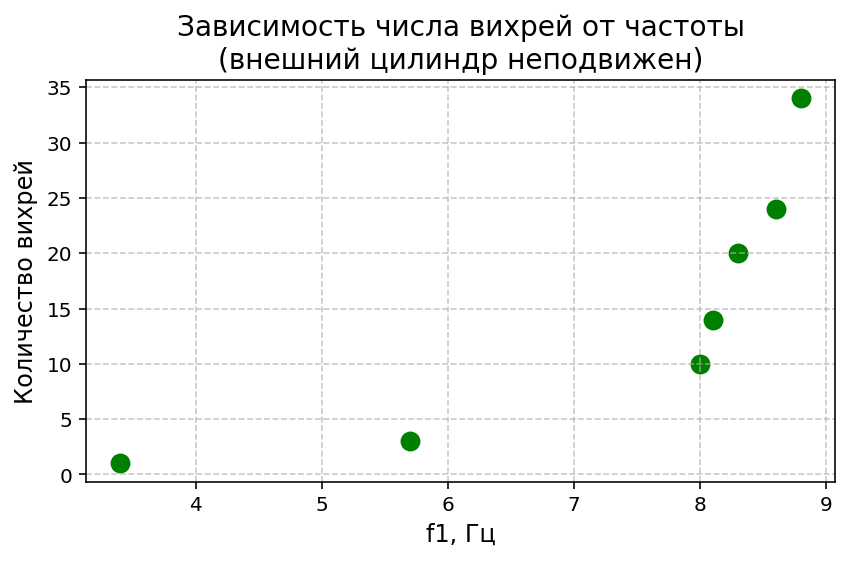
\includegraphics[scale=0.5]{photoes/f(n)1.png}
&
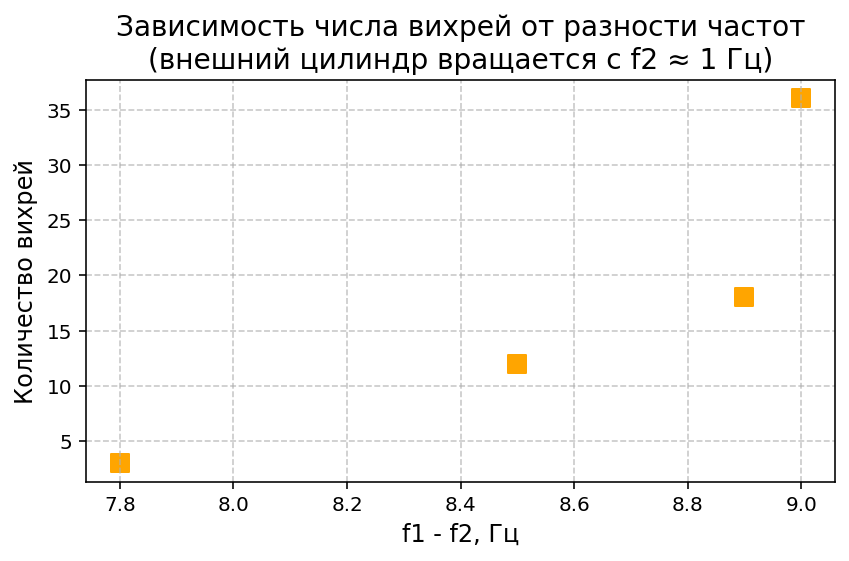
\includegraphics[scale=0.5]{photoes/f(n)2.png}
\end{tabular}
\caption{Зависимость числа вихрей от частоты вращений}
\label{Fig:Race}
\end{figure}



\subsection{Граница устойчивости}
Граница устойчивости построена по табличным значениям. Точки посчитаны из соотношений выше. Погрешность измерения частоты появления новых вихрей была оценена как 1 Гц в силу неточности измерений, погрешность кинематической вязкости указана выше и состоявляет 5%.

\begin{figure}[h]
\centering
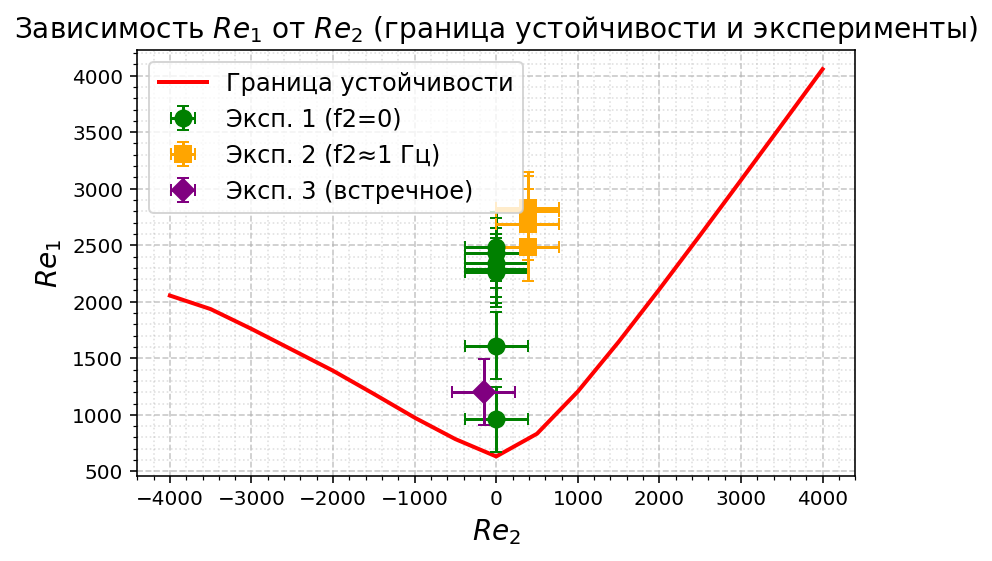
\includegraphics[width=0.65\linewidth]{photoes/Re1(Re2).png}
\caption{Зависимости Re1 от Re2}
\label{fig:mpr}
\end{figure}

\newpage
\section{Обсуждение результатов и выводы}
В ходе лабораторной работы была экспериментально исследована устойчивость течения Куэтта.

Можно сделать следующие выводы:
\begin{itemize}
    \item Количество наблюдаемых вихрей растет с ростом частоты, причем производная также растет. Можно попытаться объяснить это следующим - вихри появляются тем легче, чем неустойчивей потом. При увеличении числа вихрей возмущения растут, и чем вихрей больше, тем поток неустойчивей, поэтому требуется все меньше энергии для перехода к неустойчивости. 
    \item Все наблюдаемые точки соответствуют неустойчивому стационарному течению, причем чем меньше вихрей наблюдается, тем ближе точки к границе устойчивости.
    \item Неодновременность появления вихрей связана, вероятно, с наличием краевых эффектов на торцах цилиндра - у торцов возмущения сильнее, и переход в неустойчивый режим наблюдается раньше.
\end{itemize}

Также при движении цилиндров в разные стороны был обнаружен момент образования двух наборов вихрей. Это произошло при частотах $f1 = 4 \pm 1$ Гц, $f2 = -1\pm 1$ Гц. 

\end{document}